%%%%%%%%%%%%%%%%%%%%%%%%%%%%%%%%%%%%%%%%%%%%%%%%%%%%%%%%%%%%
%%%%%%%%%%%%%%%%%%%%%%%%%%%%%%%%%%%%%%%%%%%%%%%%%%%%%%%%%%%%
%%%%%%%%%%%%%%%%%%%%%%%%%%%%%%%%%%%%%%%%%%%%%%%%%%%%%%%%%%%%
%%%%%%%%%%%%%%%%%%%%%%%%%%%%%%%%%%%%%%%%%%%%%%%%%%%%%%%%%%%%
%%%%%%%%%%%%%%%%%%%%%%%%%%%%%%%%%%%%%%%%%%%%%%%%%%%%%%%%%%%%
\documentclass[12pt]{article}
\usepackage{epsfig}
\usepackage{times}
\renewcommand{\topfraction}{1.0}
\renewcommand{\bottomfraction}{1.0}
\renewcommand{\textfraction}{0.0}
\setlength {\textwidth}{6.6in}
\hoffset=-1.0in
\oddsidemargin=1.00in
\marginparsep=0.0in
\marginparwidth=0.0in                                                                               
\setlength {\textheight}{9.0in}
\voffset=-1.00in
\topmargin=1.0in
\headheight=0.0in
\headsep=0.00in
\footskip=0.50in                                         
\setcounter{page}{1}
\begin{document}
\def\pos{\medskip\quad}
\def\subpos{\smallskip \qquad}
\newfont{\nice}{cmr12 scaled 1250}
\newfont{\name}{cmr12 scaled 1080}
\newfont{\swell}{cmbx12 scaled 800}
%%%%%%%%%%%%%%%%%%%%%%%%%%%%%%%%%%%%%%%%%%%%%%%%%%%%%%%%%%%%
%     DO NOT CHANGE ANYTHING ABOVE THIS LINE
%%%%%%%%%%%%%%%%%%%%%%%%%%%%%%%%%%%%%%%%%%%%%%%%%%%%%%%%%%%%
%     DO NOT CHANGE ANYTHING ABOVE THIS LINE
%%%%%%%%%%%%%%%%%%%%%%%%%%%%%%%%%%%%%%%%%%%%%%%%%%%%%%%%%%%%
%     DO NOT CHANGE ANYTHING ABOVE THIS LINE
%%%%%%%%%%%%%%%%%%%%%%%%%%%%%%%%%%%%%%%%%%%%%%%%%%%%%%%%%%%%

\begin{center}
{\large
PHYSICS  30123: Observational Astronomy - Fall 2019}\\
%%%%%%%%%%%%%%%%%%%%%%%%%%%%%%%%%%%%%%%%%%%%%%%%%%%%%%%%%%%%
{\large LABORATORY X: Your Name Here}\\\vskip0.25in
%%%%%%%%%%%%%%%%%%%%%%%%%%%%%%%%%%%%%%%%%%%%%%%%%%%%%%%%%%%%
\end{center}
%%%%%%%%%%%%%%%%%%%%%%%%%%%%%%%%%%%%%%%%%%%%%%%%%%%%%%%%%%%%
% Section Heading
%%%%%%%%%%%%%%%%%%%%%%%%%%%%%%%%%%%%%%%%%%%%%%%%%%%%%%%%%%%%
\noindent {\bf PROJECT INFORMATION:} \\
% Basically an Authors List.
Collaborators: ``who you worked with, if any.''\\
% Where can I get any electronic data associated with this project. 
Data Location: ``directory where any project data/images are located''\\

%%%%%%%%%%%%%%%%%%%%%%%%%%%%%%%%%%%%%%%%%%%%%%%%%%%%%%%%%%%%
% Section Heading
%%%%%%%%%%%%%%%%%%%%%%%%%%%%%%%%%%%%%%%%%%%%%%%%%%%%%%%%%%%%
\vskip0.1in
\noindent {\bf PURPOSE:} \\

Write your text here



You can use superscripts (m s$^{-1}$) or subscripts (M$_{*}$). 




%%%%%%%%%%%%%%%%%%%%%%%%%%%%%%%%%%%%%%%%%%%%%%%%%%%%%%%%%%%%
% Bullet Point & Numbered list - lists can also be nested as below
%%%%%%%%%%%%%%%%%%%%%%%%%%%%%%%%%%%%%%%%%%%%%%%%%%%%%%%%%%%%
\begin{itemize}      % first begin-----------]
\item Item 1         %                                       
\begin{enumerate}    %       second begin----]        
\item Item a         %                              
\begin{itemize}      %           third begin-]      
\item Item c         %                     
\end{itemize}        %           third end --]  
\item Item b         %                          
\end{enumerate}      %       second end -----]  
\item Item 2         %                          
\begin{itemize}      %      fourth begin ----]  
\item Item x         %                       
\begin{enumerate}    %         fifth begin  -] 
\item Item z         %                       
\end{enumerate}      %          fifth end ---] 
\end{itemize}        %       fourth end------] 
\item Item 3         %                         
\end{itemize}        % first end ------------]

%%%%%%%%%%%%%%%%%%%%%%%%%%%%%%%%%%%%%%%%%%%%%%%%%%%%%%%%%%%%
% Section Heading
%%%%%%%%%%%%%%%%%%%%%%%%%%%%%%%%%%%%%%%%%%%%%%%%%%%%%%%%%%%%
\vskip0.1in
\noindent {\bf PROCEEDURE:} \\

Write your text here.  


%%%%%%%%%%%%%%%%%%%%%%%%%%%%%%%%%%%%%%%%%%%%%%%%%%%%%%%%%%%%
\clearpage % inserts a page break
%%%%%%%%%%%%%%%%%%%%%%%%%%%%%%%%%%%%%%%%%%%%%%%%%%%%%%%%%%%%
You can also use figures:


%%%%%%%%%%%%%%%%%%%%%%%%%%%%%%%%%%%%%%%%%%%%%%%%%%%%%%%%%%%%
% Figures can be inserted
%%%%%%%%%%%%%%%%%%%%%%%%%%%%%%%%%%%%%%%%%%%%%%%%%%%%%%%%%%%%
\begin{figure}[h!]
\begin{center}
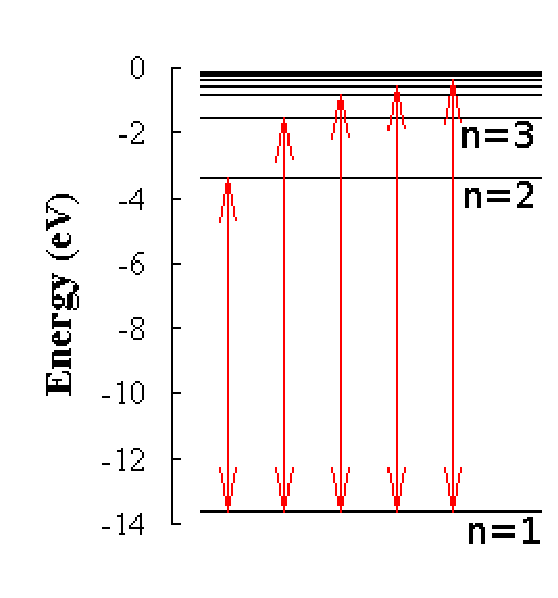
\epsfig{file=hydrogen.eps,width=2.2in}
\end{center}
\caption{This is the energy levels for the Hydrogen atom}
\end{figure}
\begin{figure}[h]
\begin{center}
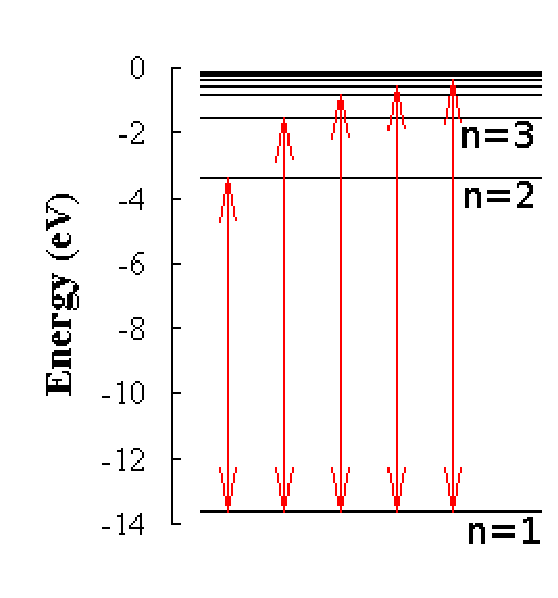
\includegraphics[scale=0.6,angle=90]{hydrogen.eps} 
\end{center}
\caption{This is the energy levels for the Hydrogen atom sideways
\label{figure:map}}
\end{figure}


\noindent {\bf ANALYSIS (and math):} \\

And go into Math mode $A_x = \int_{n-1}^{n+10}  f(x) \mathrm{d}x$ 
in the normal text or insert an equation:
\begin{equation}
	F = ma \\
	   =m \frac{dv}{dt} 
\end{equation}


or if you want to go wild:
\begin{equation}
\prod_{j\ge0}\left( \sum_{k\ge0} a_{jk}z^k \right) = \sum_{n\ge0} z^n 
\left( \sum_{k_0,k_1\ldots\ge0 \atop k_0+k_1\cdots=0} a_{0k_0} a_{1k_1}\ldots \right)
\end{equation}
and continue your text.


%%%%%%%%%%%%%%%%%%%%%%%%%%%%%%%%%%%%%%%%%%%%%%%%%%%%%%%%%%%%
% Section Heading
%%%%%%%%%%%%%%%%%%%%%%%%%%%%%%%%%%%%%%%%%%%%%%%%%%%%%%%%%%%%
\vskip0.1in
\noindent {\bf RESULTS:}\\

Write your text here.  You can also use tables to display your data.\\








%%%%%%%%%%%%%%%%%%%%%%%%%%%%%%%%%%%%%%%%%%%%%%%%%%%%%%%%%%%%
% Tables are created easily
%%%%%%%%%%%%%%%%%%%%%%%%%%%%%%%%%%%%%%%%%%%%%%%%%%%%%%%%%%%%
\begin{center}
\begin{tabular}{lcr}\hline\hline
Header 1 & Header 2 & Header 3 \\\hline\hline
Data 1a   & Data 2a   &  Data 3a    \\
Data 1b   & Data 2b  &  Data 3b    \\
Data 1c   & Data 2c   &  Data 3c    \\\hline
\end{tabular}\vskip 0.2in
\end{center}


%%%%%%%%%%%%%%%%%%%%%%%%%%%%%%%%%%%%%%%%%%%%%%%%%%%%%%%%%%%%
% Section Heading
%%%%%%%%%%%%%%%%%%%%%%%%%%%%%%%%%%%%%%%%%%%%%%%%%%%%%%%%%%%%
\vskip0.1in
\noindent {\bf CONCLUSION:}\\

Write your text here.


%%%%%%%%%%%%%%%%%%%%%%%%%%%%%%%%%%%%%%%%%%%%%%%%%%%%%%%%%%%%



\end{document}
